\documentclass[fontsize=12pt,twoside=false,numbers=noenddot]{kaobook}

\usepackage{styles/environments} % for the TODO boxes
\usepackage{expex}
\usepackage{fontspec}
\usepackage{booktabs}
\usepackage{caption}
\usepackage{subcaption}
\usepackage[utf8]{inputenc}

%--- METADATA ---%
\newcommand{\langname}{\textbf{lang2}}
\title[A Grammar of \langname{}]{\huge \langname{}}
\subtitle{grammar of a constructed language}
\author[kilenc]{\large Seth Thompson \\ \small \textit{aka} kilenc}
\date{\small \today}

%--- FORMATTING ---%
% font
\setmainfont{LibertinusSans}[Extension = .otf , Path = ./ , UprightFont = *-Regular-Custom , BoldFont = *-Bold-Custom , ItalicFont = *-Italic-Custom]
\setmonofont{Iosevka}[Scale=MatchLowercase]

% graphics
\graphicspath{{/}{images/}} % image paths

% links
\hypersetup{colorlinks=true, linkcolor=black, urlcolor=blue}

% romanization
\newcommand{\rzc}{\color{BrickRed}}
\newcommand{\rz}[1]{\textit{\rzc #1}}

% foreign words
\newcommand{\fzc}{\color[HTML]{008086}}
\newcommand{\fz}[1]{\textit{\fzc #1}}

% shortcuts for common stuff
\newcommand{\tsc}[1]{\textsc{#1}}
\newcommand{\tbs}{\textbackslash}
\newcommand{\ttd}{\char“~}
\newcommand{\tss}[1]{\textsuperscript{#1}}
\renewcommand{\bf}{\bfseries}
\renewcommand{\it}{\itshape}
\renewcommand{\sc}{\scshape}

% glossing style
\definelingstyle{gloss}{glstyle=nlevel, everyglpreamble=\bf\rzc, aboveglftskip=-8pt, belowglpreambleskip=-8pt, aboveexskip=0pt, belowexskip=-4pt}
\definelingstyle{widegloss}{glstyle=nlevel, everyglpreamble=\bf\rzc, aboveglftskip=0pt,belowglpreambleskip=0pt, aboveexskip=8pt, belowexskip=4pt}

\newenvironment{gloss}{
	\pex[lingstyle=gloss]%
}{%
	\xe%
}%

\newenvironment{gloss*}{
	\begin{minipage}{164.6mm}%
	\pex[lingstyle=widegloss]%
}{%
	\xe%
	\end{minipage}%
}%

\newcommand{\smoyd}[2]{\trailingcitation{\footnotesize \href{#1}{(\tsc{5moyd \#{}#2})}}}

\begin{document}

\frontmatter

% title page
\KOMAoptions{twoside=semi}
\maketitle
\KOMAoptions{twoside=false}

% toc
\setlength{\textheight}{23cm} % Manually adjust the height of the ToC pages
\etocstandarddisplaystyle % "toc display" as if etoc was not loaded
\etocstandardlines % toc lines as if etoc was not loaded
\tableofcontents 

% document start
\pagelayout{margin}
\setchapterstyle{kao}

% introduction
\setchapterpreamble[u]{\margintoc}
\chapter{Introduction}
\section{Origins}
\langname{} is an \emph{a priori} artlang originally conceived to fulfill a speedlang challenge, then modified to handle a relay, then finally molded into its own project. Although I had no clear motivations in mind when beginning it, I found that the confluence of random decisions---the Gleb-generated inventory, challenge stipulations, the early translation choices---made the project into something I really enjoyed.

\section{Goals}
The overarching goal is to create something I enjoy. The project is meant to be naturalistic, but when naturalism conflicts with aesthetic, aesthetic will be prioritized.

A primary way to grow this language and develop new ideas will be through translation of poetry and scientific journals. I hope that these will push the limits of my syntactical rules while also developing an interesting corpus. I'll also try to use \tsc{5moyd}s and hopefully at some point a journal to expand my ability to speak the language and get an intuitive sense for what constructions it prefers.

As I develop this conlang, my goals will be to prioritize analytic constructions (like periphraxis) over morphological ones, write in-depth documentation of how information structure manifests in the language, and ...

\section{Lore}
\langname{} is set in a worldbuilding project I create as a hobby. The language is an isolate spoken on the eastern coast of a penininsula, once the language of citystates and now a common language throughout a number of coastal countries. It is heavily influenced by East Cape, the \emph{de jure} language of the peninsula. The world the speakers know is analogous to our 1930s.

\mainmatter

\pagelayout{wide} \part{Phonology} \pagelayout{margin}

\setchapterpreamble[u]{\margintoc}
\chapter{Segments}
\section{Consonants}
\langname{} has 14 consonant phonemes, although some newer analyses also analyze voiced stops as phonemic as wells. There are four distinguished places of articulation: labial, plain alveolar, sibilant alveolar, \marginnote[*-2]{The \emph{sibilant} place of articulation is a sprachbund feature, present in other Peninsular languages including East Cape.} and dorsal. There are four distinguisheds manner of articulation: stops, fricatives, approximants, and nasals.

\begin{table}[h] \centering
    \begin{tabular}{c|cccccccc}
        \toprule
        & \multicolumn{2}{c}{\bf Labial} & \multicolumn{2}{c}{\bf Alveolar} & \multicolumn{2}{c}{\bf Sibilant} & \multicolumn{2}{c}{\bf Dorsal} \\
        \midrule
        \bf{Stop}           & p & \it\rzc p & t & \it\rzc t & t͡s & \it\rzc c & k & \it\rzc k \\
                            & (b) & \it\rzc b & (d) & \it\rzc d & (d͡z) & \it\rzc j & (g) & \it\rzc g \\
        \bf{Fricative}      & f & \it\rzc f & ɬ & \it\rzc l & s & \it\rzc s & x & \it\rzc h \\
        \bf{Nasal}          & m & \it\rzc m & n & \it\rzc m & n͡z & \it\rzc z \\
        \bf{Approximant}    & w & \it\rzc v & ɹ & \it\rzc r & & & j & \it\rzc y \\
        \bottomrule
    \end{tabular}
    \caption{Consonants}
    \end{table}

\paragraph{Nasal Sibilant}
The nasal sibilant /n͡z/ is a typologically odd segment. The prototypical representation of this sound is [z̃], a voiced fricative with simultaneous nasal release; however, phonetic research\marginnote{See \href{https://www.icacommission.org/Proceedings/ICA1998Seattle/pdfs/vol_4/2921_1.pdf}{Ohala et al. (1998)} for further discussion of nasal fricatives.} suggests that true fricatives cannot be fully nasalized. Thus, this segment's typical realization may be better represented as a slightly fricated approximant [\tss{n}z̞̃], although some speakers may realize it as a weakly nasalized [\tss{n}z] or a fully nasalized approximant [\tss{n}ɹ̃]. Nevertheless it patterns as a nasal sibilant in both distribution and allophony and is thus phonemically represented as /n͡z/.

\paragraph{Labial Fricative}
The fricative /f/ has a marginal distribution, mostly appearing in loan words and onomatopoeia. Most instances of historical /f/ underwent debuccalization and were subsequently lost. Although /x/ also appears frequently in onomatopoeia, its distribution is more widespread and it is not considered marginal.

\paragraph{Sibilant Affricate}
Although the phone [t͡s] is rather common in the corpus, its underlying form is not always the phoneme /t͡s/. \marginnote{Affrication of stop-fricative clusters and pre-[s] schwa deletion are common processes that yield [t͡s], discussed further in §\ref{sec:conso_morphono}.} The underlying phoneme is usually elucidated by inflection. For example, both \rz{tsekla} “steering wheel” and \rz{cekla} “great uncle” share the same surface form, [ˈt͡sekɬə]. However, when inflected for the plural, the former becomes [ˌtasəkˈɬaz̃əɹ] and the latter [t͡səkˈɬaz̃əɹ]. As such \rz{tsekla} is analyzed as /tasekɬa/, whereas \rz{cekla} is analyzed as /t͡sekɬa/. This analysis parallels liason in some languages.

\section{Vowels}
\langname{} has 8 vowel phonemes, 5 plain and 3 nasalized. 

\begin{table}[h] \centering
\begin{tabular}{c|cccccccccccc}
    \toprule
    & \multicolumn{4}{c}{\bf Front} & \multicolumn{4}{c}{\bf Mid} & \multicolumn{4}{c}{\bf Back} \\
    \midrule
    \bf High & i & \it\rzc i & & & & & & & u & \it\rzc u \\
    \bf Mid & e & \it\rzc e & ẽ & \it\rzc ę & (ə) & \it\rzc a & (ə̃) & \it\rzc ą & o & \it\rzc o & õ & \it\rzc ǫ \\
    \bf Low & & & & & a & \it\rzc a & ã & \it\rzc ą \\
    \bottomrule
\end{tabular} 
\caption{Vowels}
\end{table}

\begin{kaobox}[frametitle=\sc todo:]
This section about vowel neutralization probably belongs in morphophonology? It also has to do with the supersegment stress.
\end{kaobox}

\paragraph{Vowel Neutralization} 
Mid and low vowels /e a o/ and their nasal counterparts are reduced to [ə ə̃] in unstressed syllables. \marginnote[*-2]{The surface form is typically romanized \rz{a} even for underlying /e o/. Dictionaries typically denote the \emph{shadow vowels} as \rz{nbm.}, an abbreviation of \rz{nabam} “shadow.”} Schwa is not phonemic, but neutralization is common, so it appears frequently throughout the corpus. In speech, the underlying vowel becomes evident when stress is shifted due to morphological processes.

\section{Allophony}

\setchapterpreamble[u]{\margintoc}
\chapter{Supersegments}
\section{Stress}
Stress in \langname{} is lexically and morphologically productive. Stress typically falls on the penultimate syllable of a word. Atypical vowel stress, most common in loan words, is marked with an acute. \marginnote{For example, \rz{tąka} “tree” has typical stress and is unmarked, but \rz{tąká} “reindeer” has atypical ultimate stress and is thus marked.} Stress is also morphologically productive, distinguishing between unmarked and distal deixis in nouns. Affixation, compounding, and other stress-shifting processes often cause stress-based minimal pairs to become homophones.

Stressed vowels have three phonetic differences from unstressed vowels. First, they typically have a rising pitch. Second, they are typically longer than unstressed vowels. Third, onsets before long vowels have a longer VOT than other onsets, a manifestation of slight aspiration or breathiness.

Secondary stress falls on alternating syllables starting from primary stress and spreading left. For example, \rz{kagęsa} “army” has regular stress on the penultimate syllable, but when inflected in plural form, it surfaces as \rz{kegąsazar} [ˌke.gə̃ˈsa.z̃əɹ]. Secondary stress prevents the reduction of /e a o/ to [ə], but, unlike primary stress, does not cause length or VOT increase.

\setchapterpreamble[u]{\margintoc}
\chapter{Morphophonology}
\begin{kaobox}[frametitle=\sc todo:]
This all just got recently moved from allophony because it's better analyzed as a morphophonological phenomenon, probably. So some of it will have to be re-written with that framing in mind. Probably means a lot more double slashes and “it only occurs across morpheme boundaries” type stuff.
\end{kaobox}
\section{Consonants} \label{sec:conso_morphono}
\paragraph{Voicing}
Nasal and stop clusters are realized as voiced stops, occasionally prenasalized. The resulting phones [\tss{(m)}b \tss{(n)}d \tss{(n)}d͡z \tss{(ŋ)}g] are romanized \rz{b d j g}. \marginnote{These clusters assimilate in place to the stop, so /np/ surfaces as [b], not as [d].} Clusters where the nasal is the onset of a syllable, not a coda, do not assimilate, so /pn/ is still realized [pn]. 

Although the assimilation process is most common across morpheme boundaries or in loan words, voiced plosives can be found in some native morphemes. However, since these phones only occur word-medially in limited and predictable distribution, they are not tradtionally considered phonemic. \marginnote{Some scholars argue that voiced plosives are phonemic or becoming phonemic because of their presence in loan words and verb conjugations.} Most native words with voiced plosives are transparent compounds, such as \rz{ebar} “below” (← \rz{ez} + \rz{par}) or \rz{kagęsa} “army” (← reduplication of \rz{kęsa}).

Some words, especially some conjugations of \rz{m}-stem verbs, are spelled with a word-final voiced stop, but the stop is still typically realized as a medial cluster. For example, \rz{sed} “they tell me” is underlying /semt/ and realized [se\tss{(n)}d(ə)]. For some speakers, especially younger speakers or those in informal contexts, the final schwa is elided.

\begin{kaobox}[frametitle=\sc todo:]
Affrication and assibiliation would make more sense if it was only accross morpheme boundaries, but I have some words that I like where it's morpheme-internal. How should I handle that? It could be reworked as a diachronic process, made phonemic, a morphophonemic process---but it needs more thought.
\end{kaobox}

\paragraph{Affrication}
Alveolar plosive and fricative clusters are realized as a sibilant affricate. Clusters of /ts/, /tf/, /tɬ/ and /tx/ all neutralize to [t͡s], romanized as \rz{c}. The /tn͡z/ cluster likewise affricates, but is realized as [t͡s̞̃], romanized as \rz{cz}. \marginnote[*-2]{The voiceless nasal affricate is notoriously hard for non-native speakers to pronounce and is often used as a shibboleth.}

\paragraph{Assibilation}
Sibilant and non-sibilant fricative clusters are realized as sibilants. Unvoiced sibilants /t͡s s/ clustering with /f x ɬ/ are realized as [sː], romanized as \rz{cc} or \rz{ss} depending on the underlying phoneme. The voiced sibilant /n͡z/ instead is realized as [z̞̃ː] in such clusters, romanized as \rz{zz}.

\section{Vowels}
\paragraph{Schwa Deletion}
The reduced vowel [ə] is often deleted between consonants,\marginnote{Nasalized schwa [ə̃] rarely undergoes deletion as it is typically longer than [ə].} especially non-alveolar stops, and the sibilants /t͡s s n͡z/. For example, \rz{ksarat} /kosaɹat/ is commonly realized as [ksaɹət], and spelled accordingly. The elision process results in word-final or word-initial [s]\marginnote{Note that /t͡s/ surfaces [s] in these environments.} or [z̃] being the only syllable-internal clusters. However, these clusters are not consistently realized, and occasionally have an epenthetic schwa, especially word-finally. 

\begin{kaobox}[frametitle=\sc todo:] 
Something here about word-final clusters. I haven't been consistent about when it's spelled as a cluster or when it's spelled with the vowel, and I need to either commit to the inconsistency, or figure out how that works.
\end{kaobox}

\begin{kaobox}[frametitle=\sc todo:] 
There might end up being an isogloss map of schwa deletion: most dialects delete ahead of sibilants, some ahead of sibilants and approximants, and others in all environments?
\end{kaobox}

\setchapterpreamble[u]{\margintoc}
\chapter{Phonotactics}
\section{Roots}
\paragraph{Nouns}
Most nominal roots are of the form CV(C)CV. Nominal roots infrequently end in a consonant, typically /s/ or /r/ for neuter nouns. Rarely, nominal roots end in /m n/ or /k/.

\paragraph{Verbs}
Most verbal roots are of the form (C)VC or CV(C)CVC. /t/ is the most common root-final phoneme, although there are some /m/ and /r/ stems as well.

\paragraph{Affixes}
A smaller set of phonemic segments are allowed in affixes. Neither the labials /p f m w/ nor the high vowel /u/ appear in true affixes.\marginnote{Because /u/ and /w/ pattern similarly, some phonemic analyses conflate them.} In the fossilized partial reduplication process, the reflexes of labial are either /k/ (← /p f/) or /n/ (← /m w/). The high vowel /u/ lowers to /o/, often simply realized as [ə].

\section{Frequencies}
\begin{kaobox}[frametitle=WIP Lexifer file]
\begin{verbatim}
with: std-ipa-features coronal-metathesis

letters: a ą b c d e ę f g h i k l m n o ǫ p r s t u v y z 

C = t s k n y h r c m z l p v f
N = s r m n k
P = t m r
V = a e i ą o ę ǫ u

random-rate: 40
words:  CVC?CVN? C?VC?CVP C?VP C?VN?

filter: mt > d; nt > d; zt > d; mc > j; nc > j; zc > j; mk > g; nk > g; zk > g; mp > b; np > b; zp > b; ts > c; tl > c; th > c; tf > c; tz > cz; sc > ss; sl > ss; sh > ss; sf > ss; cs > cc; cl > cc; ch > cc; cf > cc; zs > zz; zc > zz; zf > zz; zl > zz; zh > zz;
\end{verbatim}
\end{kaobox}

\pagelayout{wide} \part{Morphosyntax} \pagelayout{margin}

% There are 3 primary word classes: nouns, verbs, and adpositions. There are also a limited number of adjectives and discourse particles.

\setchapterpreamble[u]{\margintoc}
\chapter{Nouns}
The \langname{} noun phrase is largely analytic, but nouns do inflect for deixis and number. Nouns have three broad inflection patterns, largely related to the way they inflect for plurality.

\section{Stems}
Nouns are broadly divided into three stems based on their inflectional patterns: \emph{vocalic}, \emph{\rz{s}-stems}, and \emph{\rz{r}-stems}. Rarely noun stems will end in other consonants, but these have no discernible shared patterns and often comprise newer loans.

Most noun stems are vocalic stems; typically these end in mid vowels, although some do end in a high vowel. Vocalic stems are usually common gender, excluding loanwords, which are prescriptively assigned neuter gender even if they end in a vowel. 

Neuter nouns, on the other hand, are often either \rz{r}-stems or \rz{s}-stems, the latter being more common. \marginnote{\rz{S}-stems can end in any sibilant, typically \rz{-s} but also \rz{-c} or \rz{-z}.} Although no longer morphologically productive, the endings on \rz{s}-stems and \rz{r}-stems derive from historical derivation processes. Many roots are reflected in both endings, but the shared meaning between them is not always transparent.

\subsection{Vocalic stems}
Vocalic stems have fairly regular, agglunative inflection patterns. However, the proximal plural is shortened to \rz{-rran} for most speakers.

\begin{table}[h] \centering
    \begin{tabular}{c|ccc}
        \toprule
        & \bf Generic & \bf Proximal & \bf Distal \\
        \midrule
        \bf \sc sg & \it\rzc metka & \it\rzc metkan & \it\rzc matkó \\
        \bf \sc pl & \it\rzc matkozar & \it\rzc matkorran & \it\rzc matkazár \\
        \bottomrule
    \end{tabular}
    \caption{Inflection of vowel-stem \rz{metka} “bowl”}
    \label{tab:metka_inflection}
\end{table}

All vocalic forms share the same endings, but many will have an unpredictable final vowel due to stress-based mid vowel neutralization. There is no way to predict the final vowel from the uninflected lemma, so learners often resort to memorization.

\subsection{Neuter stems}
Neuter stems share a common inflection pattern. For both neuter stems, the proximal surfaces as /on/ instead of /n/. The proximal plural also shortens for neuter stems, but takes the form \rz{-zza-}, influenced by the assibilation morphophonological process. The shared plural form for both stems can create homophones.\marginnote[*-2]{Some strategies to resolve homophones are covered in §\ref{subsec:additive_plural}.} 

\begin{table}[h] \centering
    \begin{tabular}{c|ccc}
        \toprule
        & \bf Generic & \bf Proximal & \bf Distal \\
        \midrule
        \bf \sc sg & \it\rzc retus & \it\rzc ratusan & \it\rzc ratús \\
        \bf \sc pl & \it\rzc ratuzzar & \it\rzc ratuzzan & \it\rzc ratuzzár \\
        \bottomrule
    \end{tabular}
    \caption{Inflection of \rz{s}-stem \rz{retus} “blade”}
\end{table}

\begin{table}[h] \centering
    \begin{tabular}{c|ccc}
        \toprule
        & \bf Generic & \bf Proximal & \bf Distal \\
        \midrule
        \bf \sc sg & \it\rzc pebar & \it\rzc pabaran & \it\rzc pabár \\
        \bf \sc pl & \it\rzc pabazzar & \it\rzc pabazzan & \it\rzc pabazzár \\
        \bottomrule
    \end{tabular}
    \caption{Inflection of \rz{r}-stem \rz{pebar} “garden”}
\end{table}

\section{Deixis}
Nominal deixis has a variety of uses, including evidentiality, distance, familiarity, and topicality.\marginnote{I had this idea, then found out that, as usual, a natural language had it first. Read \href{http://lingpapers.sites.olt.ubc.ca/files/2020/07/11_ICSNL55_Huijsmans_Reisinger_Matthewson_final.pdf}{Huijsmans, Reisinger, and Matthewson (2020)} for more about the Salishan languages.} Verbs and adjectives exhibit agreement for deictic reference. There are three deictic categories: \emph{generic}, \emph{proximal}, and \emph{distal}.

\subsection{Generic}
The unmarked or dictionary form of a noun is used when the noun is widely understood or well-known, for immaterial referents that cannot be deictically located, or if evidence of the referent is not known. If direct or reported evidence exists, it's infelicitous or questionably grammatical to use unmarked form.

\subsection{Proximal}
The proximal form of a noun is used when the speaker is certain, nearby, or familiar with the noun.
%It can also be used for the conversational topic.
This form most commonly denotes direct evidence, meaning the speaker has personal experience with the marked noun. It is marked with the suffix \rz{-n}. \marginnote[*-2]{\rz{-n} is morphophonemically ⫽on⫽, where ⫽o⫽ doesn't surface for vocalic stems.}

\paragraph{Direct evidence}
The canonical meaning of the proximal form is direct evidence, often translated as “I saw.” 

\begin{kaobox}[frametitle=\sc todo:]
    The definiteness constructions probably need to be reworked to square better with (a) the stuff I've learned about definiteness and (b) the use of the deictic forms for topic/focus.
\end{kaobox}

\paragraph{Definiteness}
Proximal forms can be used to describe the definiteness of a referent. This construction is only used for weak, uniqueness-based definiteness (eg. “the Moon”), never for strong, anaphoric definiteness (eg. “the book”). For strong definitess, the noun \rz{sin} “???” is used alongside distal form, as in (\nextx b).

\begin{gloss*}
    \a \begingl
        \glpreamble Nassoin kąstecik su kagęsa su kagę́stapa. \endpreamble
            nassoi-n[king-\tsc{prox}]
            kąstecik[command]
            su[and]
            kagęsa[army]
            su[and]
            kagę́stapa[navy]
        \glft “The king (that we know) commands both army and navy.”
    \endgl
    \a \begingl
        \glpreamble sah ez-Rosąm pít ató sín. \endpreamble
            sah[soon]
            tę=rosąm[\tsc{prep}=cook]
            pít[hold\tbs\tsc{dist}]
            ató[grain\tbs\tsc{dist}]
            sín[???\tbs\tsc{dist}]
        \glft “The rice (that you mentioned) is about to be cooked.”
        \smoyd{https://www.reddit.com/r/conlangs/comments/kck1hi/1381st_just_used_5_minutes_of_your_day/}{1381}
    \endgl
\end{gloss*}

\subsection{Distal}
The distal form of a noun is used when the speaker is uncertain, far, or unfamiliar with the noun. 
%It can also be used for the conversational focus.
This form typically denotes indirect evidence, including inference, meaning the speaker has heard of or can make an educated guess about the existence of the marked noun. Reported deixis is marked by shifting stress to the ultimate syllable of the word.

\paragraph{Indirect Evidence}
The prototypical meaning of the distal form is indirect evidence, often translated as “heard about” or “they said.” As in (\nextx), this evidence is encoded into the clause via the subject and the predicate that agrees with it.

\begin{gloss*}
    \begingl
        \glpreamble egi Matkó aczé sém lar tę-het.\endpreamble
            egi[just]
            matkó[basket\tbs\tsc{dist}]
            aczé[two\tbs\tsc{dist}]
            sém[will:be\tbs\tsc{dist}]
            lar[there]
            tę=het[\tsc{prep}=be:at]
        \glft “(She said) there will be just two baskets.”
        \smoyd{https://www.reddit.com/r/conlangs/comments/ic7on8/1314th_just_used_5_minutes_of_your_day/}{1314}
    \endgl
\end{gloss*}

\section{Number}
Nouns inflect morphologically for an additive plural, but there is also a syntactic construction used to form associative plurals. The unmarked form of a noun encodes expected number, \eg \rz{parsa} “eyes” which defaults to a pair and must be modified by a numeral or apposotive to specify a singulative. 

\begin{figure}[h]
    \centering
    \begin{subfigure}{0.4\textwidth}
        \centering
        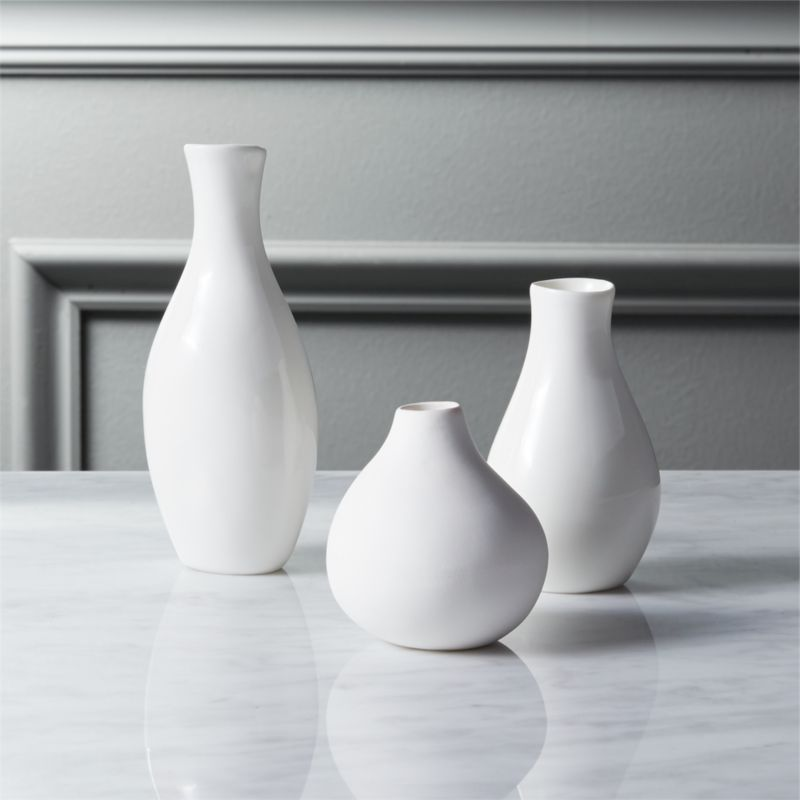
\includegraphics[width=\textwidth]{same_vases.jpg}
        \caption{\rz{matkozar}}
    \end{subfigure}
    \begin{subfigure}{0.4\textwidth}
        \centering
        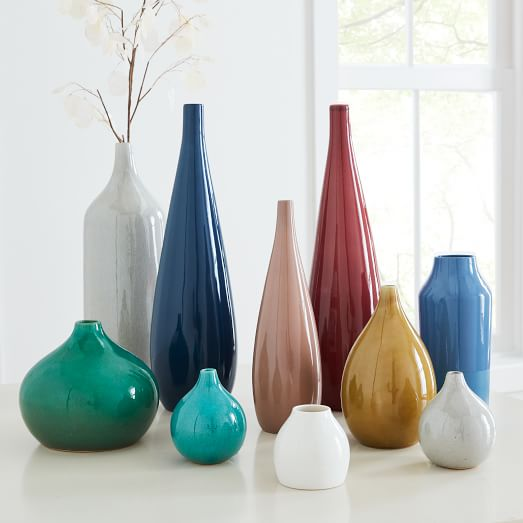
\includegraphics[width=\textwidth]{different_vases.jpg}
        \caption{\rz{ezzu metka}}
    \end{subfigure}
    \caption{Additive vs. associative plurals}
\end{figure}

The primary difference in the two plurals is the composition of the set: additive plurals refer to largely homogenous referents, whereas associative plurals refer to largely heterogenous referents.

\subsection{Additive plurals} \label{subsec:additive_plural}
Additive plurals are used for a set of homogenous referents and never heterogenous referents; \eg \rz{matkozar} is “a set of the same (or similar) bowl” and never “a set of diverse bowls.”\marginnote{The second meaning would use the associative plural.}

Additive plurality is indicated through the suffix \rz{-zar}. Morphological marking is optional and a noun can be inferred additively plural from context. \marginnote{Mandatory plural marking is stylistically preferred in formal contexts.} As such marking is less common for small, discrete or easily countable sets or when a referent has been established plural in prior conversation. However, speakers are not always consistent with marking.

Morphonologically, plural marking can be thought to precede deictic marking; plural distal nouns have accent placed on the plural suffix. As seen in Table \ref{tab:metka_inflection}, \rz{matkozar} becomes \rz{matkazár}, not \rz{*matkózar}.

\paragraph{Combating homophony}
Because the suffixes of \rz{s}-stems and \rz{r}-stems merge in the plural, some minimal pairs are rendered homphones when inflected. To combat this, speakers sometimes employ \rz{tevi} “many” as an appositive modifier for the singular form.

\paragraph{Explicit number}
When number is specified with a numeral, the noun is not marked for plurality, as in (\nextx). This can also be used as another strategy to combat homophony.

\begin{gloss}
    \begingl
        \glpreamble vęci ocza \endpreamble
            vęci[mercenary]
            ocza[two]
        \glft “two mercenaries”
        \trailingcitation (cf. \rz{vącizar} “mercenaries”)
    \endgl
\end{gloss}

\subsection{Associative plurals}
Unlike the additive plural, the associative plural is not marked morphologically; it is nonetheless rather prevalent. The preposition \rz{ezzu} conveys the associative meaning.\marginnote{Like \rz{su}, \rz{ezzu} can appear stranded. See §\ref{subsec:u_and_su}.}

The associative is used for a set of heterogenous referents. For animate (especially human) referents, the meaning is canoncically “a person and their associates,” as in (\nextx). The focal referent\marginnote{Terminology in this section adapted from \href{https://amor.cms.hu-berlin.de/~h2816i3x/Lehre/2007_VL_Typologie/03_Daniel_AssociativePlural.pdf}{Daniel and Moravcsik (2007)}.} (\ie most important) is the marked noun.

\begin{gloss}
    \begingl
        \glpreamble Sayanarnat otik ezzu Kanyi ez-laran. \endpreamble
            sayenar-nat[be.ignorant-\tsc{cvb}]
            ot-ik[be-\tsc{prox}]
            ezzu[\tsc{assoc}]
            Kanyi[\tsc{name}]
            ez=lar-n[\tsc{prep=expl-prox}]
        \glft “For this, Kanyi and his friends won't be much \emph{help}.”
    \endgl
\end{gloss}

However, the associative can also have a number of idiomatic, context-specific meanings, usually referring to diverse groups.

% \pex 
% \a \begingl
% \glpreamble ezzu Akakvazi rematt \endpreamble
% \glft “The diverse group of tag players entertained us ...”
% \endgl 
% % \a \begingl
% % \glft “My grandfather painted a wide variety of paintings.”
% % \endgl
% \xe

\section{Gender}
Although nouns traditionally distinguish \emph{common} and \emph{neuter} gender, this has largely become a prescriptive convention. \marginnote{The gender distinction is more common in literature or academia.} Loanwords, especially technical loanwords, are typically assigned neuter gender. Some words only distinguish gender for certain uses or contexts, thus dictionaries typically denote if a given usage is expected to require neuter gender.

\section{Apposition}
Apposition is fairly common due to the small adjective class present in \langname{}. Apposition is used in a number of collocative constructions but is distinct from compounding largely because of stress patterns and morphophonological processes.\marginnote{Compounds can shift stress and also show cross-morpheme sound changes.} Furthermore, appositive nouns shown agreement with the noun they modify, like adjectives.

\subsection{Inalienable possession}
Apposition is a fairly common strategy for possession of all types,\marginnote{Alienable possession via apposition is dispreferred in formal registers.} but inalienably possessed nouns require apposition, as in (\nextx b).

\begin{gloss}
    \a \ljudge{?} \begingl 
        \glpreamble  hora im-kęsa \endpreamble
        hora[wrist]
        im=kęsa[of=soldier]
        \glft \textit{Intended:} “soldier's wrist”
    \endgl
    \a \begingl 
        \glpreamble hora kęsa \endpreamble
        hora[wrist]
        kęsa[soldier]
        \glft “soldier's wrist”
    \endgl
\end{gloss}

The sentence in (\lastx a) more readily lends itself to a reading indicating inalienable possession, such as “soldier's craftmanship” or “soldier's weaponsmithing.”

\subsection{Reducing syntactic complexity}
Appositives are also used as a way of combating heaviness in complex noun phrases. This often occurs in noun phrases with multiple prepositional modifiers, especially when one of the modifiers is \rz{im} “of.” Other prepositions can be reduced this way as well. 

When multiple prepositional phrases modify a head noun the phrase is syntactically heavy. For example (\nextx) has three modifiers, an adjective and two prepositional phrases, one with its own adjective.

\begin{gloss*}
    \begingl
        \glpreamble rat Hecik pakné taá im-lalasan ez-helazzaran acoan. \endpreamble
        rat[I]
        hecik[be.at]
        pakné[house\tbs\tsc{dist}]
        taá[blue\tbs\tsc{dist}]
        im=lalasa-n[of=auntie-\tsc{prox}]
        ez=helazzaran[\tsc{prep}=mountains]
        acoan[tall]
        \glft “I'll be at auntie's blue house near the tall mountains.”
    \endgl
\end{gloss*}

To reduce the syntactic load of the sentence, a speaker might instead render it as (\nextx). The phrase is clearly appositional; \rz{lalasa} switches from proximal marking (indicating the speaker has met her) to distal marking (to agree with its head noun). 

\begin{gloss*}
    \begingl
        \glpreamble rat Hecik pakné taá lalasá ez-helazzaran acoan. \endpreamble
        rat[I]
        hecik[be.at]
        pakné[house\tbs\tsc{dist}]
        taá[blue\tbs\tsc{dist}]
        lalasá[auntie\tbs\tsc{dist}]
        ez=helazzaran[\tsc{prep}=mountains]
        acoan[tall]
        \glft “I'll be at auntie's blue house near the tall mountains.”
    \endgl
\end{gloss*}

The new sentence has fewer function words and less disparate inflections, reducing some of its complexity.

\section{Phrasal syntax}
Noun phrases are predominantly head-initial. Generally speaking, syntactically simpler consituents occur before more syntactically complex ones, as shown in (\nextx).

\begin{gloss}
    head → adjective → number → appositive → prepositional phrase
\end{gloss}

\setchapterpreamble[u]{\margintoc}
\chapter{Pronouns}
Prounouns are morphologically and syntactically similar to other nouns---they share inflectional patterns and can be modified by adjectives. The notable differences are that pronouns rarely inflect for deixis, and some appositive constructions are ungrammatical.

\begin{kaobox}[frametitle=\sc todo:]
Settle on pronominal forms---right now it's \rz{rat} \tsc{1}, \rz{a(f)} \tsc{2}, \rz{sec} \tsc{3c}, and \rz{moc} \tsc{3n}. There's some isogloss map about whether \tsc{2} is \rz{a} or \rz{af}.
\end{kaobox}

\paragraph{Possession}
Like nominal possession, pronominal possession can be expressed either through apposition or prepositional phrases. \marginnote{Formal registers prefer the prepositional construction.} Thus both \rz{lar im-sec} and \rz{lar sec} can mean “his thing.” However, apposition is more common in isolation for pronouns than it is for nouns.



\setchapterpreamble[u]{\margintoc}
\chapter{Verbs}

\begin{kaobox}[frametitle=\sc todo:]
    Like in \emph{§ Nouns}, it would be good to have an overview of stems and inflection patterns before diving into the meaning of the morphemes.
\end{kaobox}

\section{Agreement}
Verbs agree with both the deictic position of the subject noun and the person of the two least oblique arguments of transitive verbs.


\subsection{Polypersonal}
Transitive verbs exhibit polypersonal agreement via a suffix to the verb root. Intransitive verbs don't require person marking, but it can be used for emphasis or clarification; in such cases, either the reflexive or \gsc{3c} patient morpheme is used.

%\begin{table}[h] \centering
%\begin{tabular}{cc|cccc}
%	& & \multicolumn{4}{c}{\textbf{Patient}} \\
%	& & \textbf{1} & \textbf{2} & \textbf{\gsc{3c}} & \textbf{\gsc{3n}} \\ \hline
%	\multirow{5}{*}{\textbf{Agent}} & \textbf{1} & - & c & s & n \\
%	& \textbf{2} & t & - & s & n \\
%	& \textbf{\gsc{3c}} & t & s & s & n \\
%	& \textbf{\gsc{3n}} & n & z & z & z \\
%	& \textbf{\gsc{refl}} & \multicolumn{4}{c}{k} \\
%\end{tabular}
%\caption{Person agreement}
%\end{table}

\begin{table}[h] \centering
\begin{tabular}{cc|cccc}
	& & \multicolumn{4}{c}{\textbf{Patient}} \\
	& & \textbf{1} & \textbf{2} & \textbf{\gsc{3c}} & \textbf{\gsc{3n}} \\ \midrule
	\multirow{5}{*}{\textbf{Agent}} & \textbf{1} & - & c\cellcolor{purple!25} & s\cellcolor{yellow!25} & n\cellcolor{blue!25} \\
	& \textbf{2} & t\cellcolor{green!25} & - & s\cellcolor{yellow!25} & n\cellcolor{blue!25} \\
	& \textbf{\gsc{3c}} & t\cellcolor{green!25} & s\cellcolor{yellow!25} & s\cellcolor{yellow!25} & n\cellcolor{blue!25} \\
	& \textbf{\gsc{3n}} & n\cellcolor{blue!25} & z\cellcolor{red!25} & z\cellcolor{red!25} & z\cellcolor{red!25} \\
	& \textbf{\gsc{refl}} & \multicolumn{4}{c}{k\cellcolor{black!25}} \\
\end{tabular}
\caption{Person agreement}
\end{table}

Because many agreement suffixes share the same form, \langname{} is only occasionally pro-drop.

\subsection{Deictic}
Generic noun forms do not have agreement morphemes, but proximal nouns demand the verbal suffix \rz{-ik} and distal nouns demand the verbal suffix \rz{-ǫ}. These suffixes are attached after polypersonal agreement suffixes.

\section{Negation}
Negation ...

The negative verb suffix is \rz{-res}. \marginnote{The affix's position is from its origin as an auxiliary which bore agreement.} It occurs before agreement affixes.

\section{Converb}
The converb form of a verb is used for simultaneous action. The converb is commonly used to describe the manner of the main clause, and is also commonly used in periphrastic constructions.

The converbial suffix is \rz{-nat}.

\section{Transitivity}
Transitivity is lexically fixed, but transitive verbs can still be functionally intransitive with the use of dummy objects.

Prescriptive convention holds that verbs exhibit polypersonal agreement with their dummy objects, but speakers commonly omit polypersonal marking in these constructions, as in (\nextx b).

\pex
\a \begingl
\glpreamble sec Sasamsik tasa. \endpreamble
sec[\gsc{3c}]
sesam-s-ik[say-\gsc{3c.p-prox}]
tasa[letter]
\glft “He's saying something.”
\trailingcitation (Formal)
\endgl
\a \begingl
\glpreamble sec Semik lar. \endpreamble
sec[\gsc{3c}]
sem-ik[say-\gsc{prox}]
lar[\gsc{exp}]
\glft “He's talking.”
\trailingcitation (Informal)
\endgl \marginnote[*-3]{Informal constructions often use the more grammaticalized \rz{lar} instead of the dummy collocative.}
\xe

Not every verb has a collocated intransitive form. For these verbs, periphrastic constructions can also serve as valency-changing operations.

\section{Periphraxis}
Periphrastic constructions handle most temporal marking in \langname{}, covering aspects and moods. The core verb of the periphrastic construction is the only finite verb of a clause, bearing all agreement, and the semantic verb is demoted to an adjunct in converbial form or as a bare infinitive with an adpositional clitic.

\subsection{\textit{ot}}
The verb \rz{ot} “be” has two periphrastic constructions, a \emph{perfective} and a \emph{support} construction used for focus-fronting verbs.

\paragraph{Perfective}
In the perfective construction, the semantic verb is demoted to adjunct with the preposition \rz{tę}.

\paragraph{Support}
In the support construction, the semantic verb is demoted to adjunct as a converb.

\subsection{\textit{sesam}}
The verb \rz{sesam} “say” has one periphrastic construction, an irrealis.\marginnote{\rz{Sesam} is often shorted to \rz{sem} informally.}

\paragraph{Irrealis}
In the irrealis construction, the semantic verb is demoted to adjunct with the preposition \rz{tę}. 

\subsection{\textit{nenat}}
The verb \rz{nenat} “” has one periphrastic construction, a subjunctive.

\paragraph{Subjunctive}
In the subjunctive construction, the semantic verb is demoted to adjunct with the preposition \rz{ah}. The subjunctive construction has a more limited scope than the \rz{sesam} irrealis construction, typically expressing counterfactuals or doubt.

\subsection{\textit{het}}
The verb \rz{het} “be at” has two periphrastic constructions, a \emph{passive} and an \emph{imperfective}, the latter typically restricted to narrative contexts.

\paragraph{Passive}
In the passive construction, the semantic verb is demoted to adjunct as a converb. The \rz{het} passive is not a true passive because the verb does not change valency (\ie the \gsc{a}-like argument cannot be omitted). Instead of valency operations, the role of this construction is typically to change verbal agreement, as in (\nextx).

\begin{gloss*}
\a \ljudge{*} \begingl
\glpreamble Azzár hossusarsik nassoin.\endpreamble 
as-zár[foreigner-\gsc{pl.dist}]
hassusar-s-ik[exalt-\gsc{3c»3c-prox}]
nassoi-n[king-\gsc{prox}]
\glft \textit{Intended:} “(I see) the foreigners (I've heard about) praising the king.”
\endgl
\a \begingl
\glpreamble Nassoin hecik azzár hossusarnat.\endpreamble
nassoi-n[king-\gsc{prox}]
het-s-ik[be.at\gsc{-3c»3c-prox}]
as-zár[foreigner-\gsc{pl.dist}]
hassusar-nat[exalt-\gsc{cvb}]
\glft “(I see) the king being praised by the foreigners (I've heard about).”
\endgl
\end{gloss*}

In (\lastx a), the hypothetical speaker intends to mark the verb as proximal to convey direct evidence, but the utterance is ungrammatical because the verb doesn't agree with its subject, \rz{azzár}. To correct this, the construction in (\lastx b) is used, which takes advantage of the passive to mark the verb phrase as proximal.

\par In addition to its role shuffling agreement, the \rz{het} passive can also be used to clarify sentences that become ambiguous due to focus fronting, as in (\nextx).

\begin{gloss*}
\a \begingl
\glpreamble Kanyin akakvatcik Arpatan. \endpreamble
Kanyi-n[\gsc{name-prox}]
akekvat-s-ik[tag-\gsc{3c»3c-prox}]
Arpat-n[\gsc{name-prox}]
\glft “Kanyi tagged Arpat.” \\ \textit{or} “Who Arpat tagged was Kanyi.”
\endgl
\a \begingl
\glpreamble Kanyin hecik Arpatan akakvatnat. \endpreamble
Kanyi-n[\gsc{name-prox}]
het-s-ik[be.at\gsc{-3c»3c-prox}]
Arpat-n[\gsc{name-prox}]
akekvat-nat[tag-\gsc{cvb}]
\glft “Kanyi was tagged by Arpat.”
\endgl
\end{gloss*}

In (\lastx a), it's not clear if Kanyi is the semantic agent or a semantic patient that's been fronted for focus. Without context, both interpretations are grammatical. The use of the passive in (\lastx b) is less ambiguously interpreted, almost always meaning that Arpat was the semantic agent.

\subsection{\textit{pit}}
\begin{kaobox}[frametitle=\sc todo:]
    Rework the \rz{pit} passive, which currently doesn't make a lot of sense--how is it demoting stuff, when semantically you'd expect “hold” to be transitive? Maybe \rz{pit} means something else, maybe it will demote in a different way, maybe the valency is weirder...
\end{kaobox}
The verb \rz{pit} “hold” has one periphrastic construction, the mediopassive. \marginnote[*-2]{Unlike most other periphrastic verbs, \rz{pit} is rarely used outside periphrasis, having largely been replaced by \rz{akrar}.}

\paragraph{Mediopassive}
In the mediopassive construction, the semantic verb is demoted to adjunct with the preposition \rz{ez}. Unlike the \rz{het} passive, the \rz{pit} mediopassive is a true passive; the \gsc{a}-like argument does not appear.


\setchapterpreamble[u]{\margintoc}
\chapter{Adpositions}
Adpositions are syntactically bound morphemes that express some relationship (often spacial) between constituents. However, they are considered words, not affixes, because the stress pattern of the noun they bind to does not shift. \marginnote{Compare \rz{kąsazar} “soldiers,” marked via affix, to \rz{retus im-kęsa}, “soldier's blade,” marked via adposition.} Their phonological independence differentiates them from affixes.

Adpositions are a closed class, composed of only 5 members; finer distinctions can be made with periphrastic constructions, such as \rz{tę-kamc im} “after, to the back of.” Although many such constructions are common enough to be lexically set, they are not nearly as ubiquitous as lone prepositions.

\subsection{\textit{im}}
The adposition \rz{im} indicates possession.

\subsection{\textit{ez}}
The adposition \rz{ez} conveys location inside an object or large body.

\subsection{\textit{tę}}
The adposition \rz{tę} conveys motion relative to a location, either towards or away from.

\subsection{\textit{ah}}
The adposition \rz{ah} conveys location on the surface of another object.

\subsection{\textit{osc}}
The adposition \rz{osc} conveys location surrounding another object. It is commonly used in a temporal sense to indicate a time frame, often translated as “around the time of.”

\setchapterpreamble[u]{\margintoc}
\chapter{Adjectives}

\setchapterpreamble[u]{\margintoc}
\chapter{Particles}

\setchapterpreamble[u]{\margintoc}
\chapter{Clauses}
Although the base-generated word order in \langname{} is SVO, this order rarely surfaces due to aggressive focus fronting. The most proximal, most newsworthy information is placed in the front of an utterance in first position. As a consequence, \langname{} is V2 order, mandating that a finite verb always be in second position. Adjuncts, including demoted verbal constructions, typically come after the core arguments of the verb. \marginnote{In practice, the most common word order in declarative sentences is SXOV or VXOS.} Often, however, the order of elements in a clause is determined by focality and evidentiality.

\section{Fronting}
The most likely phrases to be fronted are proximal or directly evident noun phrases,\marginnote{Often, the fronted element will be the conversational focus.} followed by distal or indirectly evident noun phrases. Generic noun phrases are rarely fronted except in fixed constructions.

\langname{} doesn't have explicit role-marking, so it's not always clear if a fronted noun phrase is subject or object. Various structures, including verb agreement and passives, help provided redundancy when context is not enough.

\section{Extraposition}
When a content-heavy phrase needs to be fronted, a dummy noun is often used to allow right-branching extraposition. The dummy noun is lexically dependent, but the generic nouns \rz{lar} or \rz{manc} can also be used, although they may sound stilted for some verbs.

\begin{gloss*}
    \begingl
        \glpreamble osc Armę́ kirąyamik isyusan ocoan im nassoi kęstat ezzar vęci. \endpreamble
            osc[\tsc{prep}]
            armę́[\tsc{dmy}]
            kirąyamik[investigate]
            {isyusan ocoan}[special:tribune]
            im[\tsc{prep}]
            nassoi[king]
            kęstat[lead]
            ezzar[\tsc{assoc}]
            vęci[mercenary]
        \glft “What the special tribune is investigating is the king's use of mercenaries.”
    \endgl
\end{gloss*}

%\xe
%\begingl
%\glpreamble \endpreamble
%???[\tsc{expl}]
%risk-ǫ[\tsc{aux.neg-dist}]
%???[2]
%???[be.familiar]
%how-to[subj-clause]
%???-ya[friend-\tsc{prox}]
%???[go]
%???[to.here]
%???=im=tę[house=\tsc{poss=prep}]
%rat[1]
%\glft “It's someone you don't know, the friend that will come to our house.”
%\smoyd{https://www.reddit.com/r/conlangs/comments/ithoza/1330th_just_used_5_minutes_of_your_day/}{1330}
%\endgl
%\xe

% \pagelayout{wide} \part{Pragmatics} \pagelayout{margin}

\pagelayout{wide} \part{Appendix} \pagelayout{margin}

\appendix

% --- COMMANDS ---
\makeatletter
\define@key{entry}{nbm}[]{\def\entry@nbm{#1}}
\define@key{entry}{pos}[]{\def\entry@pos{#1}}
\define@key{entry}{etym}[]{\def\entry@etym{#1}}
\define@key{entry}{note}[]{\def\entry@note{#1}}

\setkeys{entry}{nbm,pos,etym,note}

\newcommand{\entry}[3][]{%
\begingroup%
\setcounter{sense}{1}%
\setkeys{entry}{#1}%
\par \begin{minipage}{\columnwidth}%
	\textbf{\rzc #2}%
	\enskip {\footnotesize \ifdefempty{\entry@nbm}{}{• \entry@nbm{} nbm.} \ifdefempty{\entry@pos}{}{• \entry@pos}} \\%
	\ifdefempty{\entry@note}{}{\enskip {\footnotesize \textit{note:} \entry@note} \\}%
	\ifdefempty{\entry@etym}{}{\enskip {\footnotesize ← from \entry@etym} \\}%
	#3\vspace{12pt}%
\end{minipage}%
\endgroup%
}

% linear (digital-style) definitions
%\newcounter{sense}
%\NewDocumentCommand{\sense}{o}{%
%\ifnum\the\value{sense}>1\\\fi%
%	\textbf{\arabic{sense}:}\enskip%
%	\IfNoValueTF{#1}{}{\textit{#1}}%
%\stepcounter{sense}%
%}

% cramped (print-style) definitions
\newcounter{sense}
\NewDocumentCommand{\sense}{o}{%
\ifnum\the\value{sense}>1\enskip\fi%
	\textbf{\arabic{sense}}\enskip%
	\IfNoValueTF{#1}{}{\textit{#1}}%
\stepcounter{sense}%
}

%\define@key{mean}{use}[]{\def\mean@use{#1}}
%\define@key{mean}{jrgn}[]{\def\mean@jrgn{#1}}
%
%\setkeys{mean}{use,jrgn}

%\newcommand{\sense}[1][]{%
%\begingroup%
%\setkeys{mean}{#1}%
%\ifnum\the\value{sense}>1\\\fi%
%	\textbf{\arabic{sense}:}\enskip%
%	\ifdefempty{\mean@jrgn}{}{\textsc{\mean@jrgn} \ifdefempty{\mean@use}{}{\enskip}}%
%	\ifdefempty{\mean@use}{}{\textit{\mean@use}}%
%\stepcounter{sense}%
%\endgroup%
%}

\newenvironment{dic}[1]{%
	%\newpage%
	\addsec{#1}%
	\begin{multicols}{2}%
}{%
	\end{multicols}%
}%

\makeatother

\pagelayout{margin}
\setchapterpreamble[u]{\margintoc}
\chapter{Lexicon}
A \langname{}-to-English dictionary is provided below.

\section*{How to use}
Entries for lexical items are listed by their spelling in generic form, ignoring morphological alterations. Derived words are listed as separate entries, but their source word is given. On the other hand, idiomatic or fixed expressions are given under the lexical item.

Morphophonological information, such as \rz{nebam} vowels, underlying form, or irregular alterations, is listed when pertinent. Furthermore, senses that are specific to a certain word form are given in \textit{italics}, where as sense that are specific to a field or context are given in \textsc{\textit{small caps}}.

\section*{Examples}
Examples are generally given as simple declarative sentences, avoiding where possible movement due to focus fronting. Typically examples are chosen to provide context or illustrate usage notes for a definition.

\pagelayout{wide}
\setlength{\columnsep}{30pt}

% ===== A =====
\begin{dic}{A}
\entry[pos=n.,etym=Classical Cape \fz{dahēs} “pee”]{adahę́s}{\sense[uncountable] sand; cf. \emph{countable} \rz{sifa} “grain of sand” \sense[idiom.] citizens (of a nation, state), subjects, followers (of a leader, celebrity) \sense[\rz{ez-adahę́s}] the public, the people of a place: \rz{Natra ez-adahę́s} “the Natran indigenous peoples”}
\entry[pos=pronoun]{af}{\sense you, your, yours}
\entry[pos=n.,etym=Classical Cape \fz{gamrī}]{agąrę́}{\sense[\sc sailing] star}
\entry[pos=n.,etym=Classical Cape \fz{gamrka} “navigator”]{agątka}{\sense cartographer}
\entry[pos=n.]{ahka}{\sense 2 feet}
\entry[pos=v. tr.,etym=redup. of \rz{akvat}]{akakvat}{\sense (in a game) tag}
\entry[pos=n., etym=\rz{akakvat} + \rz{-zi}]{akakvazi}{\sense tagplayer (usually professional)}
\entry[pos=n.]{almani}{\sense wave \sense[idiom.] influence \sense[\sc politics] soft power}
\entry[pos=v. tr.]{akrar}{\sense give \sense[(reflexive)] hold, have}
\entry[pos=n.,etym=Classical Cape \fz{as} “man”]{as}{\sense foreigner}
\entry[pos=n.]{assoi}{\sense weeb for Classical Cape culture}
\entry[pos=n.]{azyam}{\sense plant, sow (crops) \sense[idiom.] give birth to}
\end{dic}

% ===== Ą =====
\begin{dic}{Ą}
\end{dic}

% ===== C =====
\begin{dic}{C}
\entry[pos=v. tr.]{cam}{\sense put (smn.) to sleep \sense[refl.] go to bed \sense[mediopassive] nap, snooze: \rz{piran picik camnat tę-kamc im-pebar} “the child napped after school.” \sense[idiom.] calm (smn.) down, soothe \sense[coll.] bore (an audience): \rz{ah-turya cad nakraran orran im-remaczi} “the comedian's subpar performance last night bored me.”}
\entry[pos=n.]{cǫca}{\sense daytime sky}
\entry[pos=n., nbm=ǫ]{cunvarą}{\sense seagull \sense[\tsc{politics}] columnist, writer (in newspaper, magazine): \rz{cunvarǫzar hazeklam tę nassoin kesaratnik lar orra} “writers critiqued the king's subpar response.” \sense[idiom. arch.] court jester; a traditional storyteller who served as a royal advisor representing the general public \sense[{\bf\rzc satat cunvarą} pej.] feign interest for attention, virtue signal}
\end{dic}

% ===== E =====
\begin{dic}{E}
\entry[pos=v. tr.]{eccut}{\sense hurt (smth.) physically; note: more severe than \rz{ęrvat} \sense[reflexive] get in an accident \sense[idiom.] surprise (smn.)}
\entry[pos=particle]{egi}{\sense (expressing disagreement or disbelief) just, only: \rz{egi Matkó aczé sém lar tę-het} “she said there'll be just two baskets.”}
\entry[pos=n.]{emas}{\sense[ntr.] plot of land}
\entry[pos=n.,nbm=ę]{ennąt}{\sense develop into, become \sense change into (a pair of clothes) \sense move to (another place)}
\entry[pos=adj.]{esyi}{\sense good \sense correct, appropriate}
\end{dic}

% ===== Ę =====
\begin{dic}{Ę}
\entry[pos=v. tr.,note=often \rz{ęrrat} for younger speakers]{ęrvat}{\sense hurt (smn.) physically or emotionally}
\end{dic}

% ===== F =====

% ===== H =====
\begin{dic}{H}
\entry[pos=n.]{hakra}{\sense battle, skirmish \sense[pl.] conflict, campaign \sense[pl.] semester, trimester, school year}
\entry[pos=v. tr., etym=redup. of \rz{husar} “shout”]{hassusar}{\sense (esp. of a leader) exalt} \sense[adj.] famous, well-known
\entry[pos=v. in.]{hazeklam}{\sense give criticism to \rz{tę} something}
\entry[pos=n.]{helas}{\sense[ntr.] mountain}
\entry[pos=v. tr.]{het}{\sense be at \sense be, exist}
\entry[pos=n.]{hora}{\sense wrist \sense[idiom.] craftmanship, handiness}
\entry[pos=v. tr.]{husar}{\sense shout at \sense praise, compliment}
\end{dic}

% ===== I =====
\begin{dic}{I}
\entry[pos=n.]{ihaiha}{\sense donkey, mule \sense[adj. pej.] dumb}
\entry[pos=n.]{isyus}{\sense[ntr.] shield \sense[\textsc{culinary} ntr.] apron \sense[\textsc{military} pl.] elite, highly trained soldiers; royal guard, special forces, black ops: \rz{pursę́ im-ǫkassoi ksarac isyuzzar} “the special forces respond to bank robberies.”}
\end{dic}

% ===== K =====
\begin{dic}{K}
\entry[pos=n.,note=underlying {/kamat͡s/,} often {[kams]} but {[kad͡z(ə)]} for some speakers]{kamc}{\sense back; the part of the body opposite the face below the neck and above the thigh, including the buttocks \sense[\rz{tę-kamc im}] after}
\entry[pos=n.,etym=redup. of \rz{kęsa} “soldier”]{kagęsa}{\sense battalion, unit \sense (as a branch of the military) army}
\entry[pos=n.,etym=analogy with \rz{kagęsa} and \rz{kę́stapa}]{kagę́stapa}{\sense (as a branch of the military) navy}
\entry[pos=n.]{kęsa}{\sense soldier \sense[\sc academic] (of a literary work) protagonist, hero \sense[archaic] slave, conscript}
\entry[pos=n.,etym=\rz{kat} “pull” + \rz{-akz}]{katakz}{\sense[\rz{katakz im-saycezzar}] butterfly effect}
\entry[pos=n.,etym=\rz{kęsa} “soldier” + \rz{-soi}]{kęsasoi}{\sense high-ranking general \sense (with specifier) military officer: \rz{kęsasoi ???} “field officer,” \rz{kęsasoi ???} “medical officer”}
\entry[pos=n.,etym=\rz{kęsa} “soldier” and \rz{taspa} “sea”]{kę́stapa}{\sense navy officer, sailor (on a military ship)}
\entry[nbm=e,pos=v. tr.]{kęstat}{\sense lead \sense[\sc military] be in command of: \rz{nassoin kąstecik su kagęsa su kagę́stapa} “the king commands both army and navy.” \sense train (an apprentice) in \rz{tę} a skill: \rz{tę-caradá kąstettik rat lalasa} “auntie's teaching me to sew.” \sense formally teach, school (a student) in \rz{ez} a discipline: \rz{rabahan picik kąstetnat ez-latya} “the minister was brought up in the faith.” \sense[pej.] indoctrinate}
\entry[pos=n.,etym=partial reduplication of \rz{pira} “child”]{kipira}{\sense adolescent; someone around or older than 8 years old who has not yet been ritually scarred}
\entry[pos=n.]{kotus}{\sense divinity}
\entry[pos=n.,etym=\rz{kotus} + \rz{-soi}]{kotussoi}{\sense body part; soul; the perfect implements wielded by an imperfect mind}
\entry[pos=v. in.]{kirǫyam}{\sense delve \sense descend deeper with forward motion into \rz{osc} some terrain (water, caves) to search for \rz{tę} something: \rz{tę-rasar kirąyamik osc-taspa} “he's swimming into the sea to search for rare fish.” \sense[\sc politics] conduct an investigation into \rz{osc} a topic: \rz{osc lar kirąyamik isyusan ocoan im nassoin kęstat ezzar vęci} “the special tribune is investigating the king's use of mercenary forces.” \sense[\rz{kirǫyam osc saycer}] wish for good luck for \rz{tę} someone: \rz{tę-af kirǫyam osc saycer tę-makra im-hakra} “good luck this semester!”}
\entry[pos=v. tr.]{ksarat}{\sense[\sc military] handle, respond to}
\entry[pos=n.]{ksofa}{\sense deciduous tree \sense growth, development (of the mind, socially)}
\end{dic}

% ===== L =====
\begin{dic}{L}
\entry[pos=n.]{lalasa}{\sense[\tsc{kinship}] great aunt \sense godmother \sense[affectionate] mentor}
\entry[pos=n.]{latya}{\sense religion}
\entry[pos=n.]{lar}{\sense[ntr.] thing; a generic dummy noun used in many constructions}
\entry[pos=n.]{lǫya}{\sense shin; the part of the body above the foot and below the thigh, including the knee and upper ankle \sense[archaic] moment, instance (of time)}
\end{dic}

% ===== M =====
\begin{dic}{M}
\entry[pos=n.]{makra}{\sense chest; the part of the body below the neck and above the groin, including the shoulders and upper arms \sense[idiom.] responsibility, maturity, calmness under pressure \sense[\rzc\bf tę-makra im] during, for the duration of}
\entry[pos=n.]{mas}{\sense[ntr.] hour \sense[\rz{tę-kamc im-mas} adv.] in an hour: }
\entry[nbm=o,pos=n.]{metka}{\sense rounded semi-circle hollow container; bowl, basket, vessel  \sense measure word for crops or farm animals}
\end{dic}

% ===== N =====
\begin{dic}{N}
\entry[pos=n.,etym=\rz{nakrat} “” + \rz{-r}]{nakrar}{\sense performance (on stage)}
\entry[pos=n.,etym=\rz{naf} “gem” + \rz{-soi}]{nassoi}{\sense king \sense royal family member, noble}
% \entry[pos=n.,etym=\rz{nassoi} “king” + \rz{-j} fossilized collective suffix,note=often {[nəsːojd͡z(ə)]}]{nassoij}{\sense aristocrat, bourgeois \sense[archaic] royal court, royal advisors}
\entry[pos=n.]{Natra}{\sense the mountain range that runs down the middle of the continent}
\entry[pos=v. tr.]{nenat}{\sense crouch, squat \sense duck below (smth.) \sense[\rzc\bf nenat ah] might, possibly; dubtative irrealis construction}
\entry[pos=n.,etym=Old East Cape]{nęcta}{\sense[\tsc{medical}] lung}
\entry[pos=n.]{nik}{\sense flat surface, plane \sense[adj.] flat}
\entry[pos=v. in.,nbm=o,etym=\rz{nik} “flat” + \rz{hor} “craft”]{nikhar}{\sense to create a map of \rz{ez} a region}
\entry[pos=n.,etym=\rz{nikhar} “make maps” + \rz{rabaha} “minister”]{níkharkah}{\sense geography \sense[archaic] cartography}
\entry[pos=n.,etym=\rz{níkharkah} “geography” + \rz{-soi}]{nikhorkassoi}{\sense geographer \sense[archaic] cartographer}
\end{dic}

% ===== O =====
\begin{dic}{O}
\entry[pos=adj.,nbm=o,note=underlying /ot͡soa/]{oca}{\sense deep \sense (of people) tall and thin, wiry, spindly}
\entry[pos=n.,nbm=e]{ocza}{\sense two}
\entry[pos=n., nbm=o]{okva}{\sense valley}
\entry[pos=adj.]{orra}{\sense dry \sense (of food) stale \sense (of people) feeble, frail \sense (of man-made objects) subpar, fragile, poorly-made}
\entry[pos=n.,nbm=o,etym=Classical Cape]{armę́}{\sense ocean}
\entry[pos=v. in.]{ossat}{\sense (of plants) to grow in size \sense (of people) to develop emotionally, intellectually}
\entry[pos=n.]{ossaczi}{\sense nurterer, gardener \sense[idiom.] caretaker, guardian¸ nanny, babysitter}
\entry[pos=v. tr.]{ot}{\sense be smth. \sense[\rzc\bf ot tę] have done \rz{tę} something; perfective construction \sense[\rzc\bf ot satatakc] do; support construction to move adjuncts}
\end{dic}

% ===== Ǫ =====
\begin{dic}{Ǫ}
\entry[pos=n.]{ǫkas}{\sense[ntr.] payment}
\entry[pos=n.,etym=\rz{ǫkas} “payment” + \rz{-soi}]{ǫkassoi}{\sense bank}
\entry[pos=particle]{ǫm}{\sense please; imperative particle}
\end{dic}

% ===== P =====
\begin{dic}{P}
\entry[pos=n.,nbm=e]{pakna}{\sense house, shelter}
\entry[pos=n.]{paltoja}{\sense winter \sense drought, dry spell \sense[\tsc{politics} idiom.] lame-duck period}
\entry[pos=n.]{parka}{\sense rainstorm}
\entry[pos=n.]{parsa}{\sense a pair of eyes \sense[idiom.] open-mindedness, understanding}
\entry[pos=n.]{pebar}{\sense garden \sense orchard \sense primary school}
\entry[pos=n.]{pira}{\sense child; someone around or under 8 years old who hasn't yet been brought fishing}
\entry[pos=v. tr.]{pit}{\sense hold, have \sense own, possess \sense maintain (a pose, viewpoint)}
\entry[pos=n.]{polars}{\sense evergreen tree}
\entry[pos=n.,etym=Old Cape \fz{purcī} “plan”]{pursę́}{\sense robbery, heist}
\end{dic}

% ===== R =====
\begin{dic}{R}
\entry[pos=n.]{rabaha}{\sense[\sc religion] minister \sense[archaic] ministry}
\entry[pos=n.,nbm=e,etym=Old East Cape \fz{raxir} “fish”, note=sometimes spelled {\rz{raxir}, pronounced {[ɹaʃɛɹ]}, in elite circles or when exaggerating}]{rasar}{\sense meat (food) \sense[archaic] fish delicacy}
\entry[pos=n.]{recam}{\sense ritual scar made by a ceremonial blade on the upper arm near the shoulder of the dominant hand (historically on only the right arm) which symbolizes adulthood; usually done around the age of 16}
\entry[pos=pronoun]{rat}{\sense me, I, my, mine}
\entry[pos=n.,etym=\rz{recam} + \rz{-c}]{recaj}{\sense adulthood \sense the human condition, humanity, humanness}
\entry[pos=n.]{retus}{\sense[ntr.] blade \sense[\sc geography] canal}
\entry[pos=n., etym=\rz{remat} “” + \rz{-zi}]{remaczi}{\sense comedian}
\entry[pos=n.]{rosa}{\sense three}
\end{dic}

% ===== S =====
\begin{dic}{S}
\entry[pos=n.]{samni}{\sense[\sc geography] horn}
\entry[pos=n.,etym=Classical Cape \fz{sapa} “hunting dog”]{sapa}{\sense hunter}
\entry[pos=n.,etym=Old East Cape]{saska}{\sense[\tsc{medical}] heart}
\entry[pos=v. in.]{sayenar}{\sense be ignorant, uninformed, unknowledgeable about \rz{ez} a topic: \rz{ sayanarnat ez-latya tahątresik asan ah-mas esyi} “ignorant of the religion, the foreigner didn't pray at the correct hour.” }
\entry[pos=n., etym=\rz{secyat} “shine” + \rz{-r}]{secyar}{\sense celestial object: sun, moon, star \sense[\rz{sayceran im-turya}] the Moon \sense[\rz{saycer tea}] moon, satellite}
\entry[pos=n., etym=\rz{secyar} “star” + \rz{rabaha} “minister”]{sécyarkah}{\sense astronomy}
% \entry[pos=n.,etym=\rz{sécyarkah} “astronomy” + \rz{-soi}]{sacyerkassoi}{\sense astronomer}
\entry[pos=n.]{senva}{\sense eight}
\entry[pos=v. tr.,note=often shortened to \rz{sem}]{sesam}{\sense say (smth.) \sense hope for, wish for (smth.) \sense[\rzc\bf sesam tę] may, might, possibly; irrealis construction}
\entry[pos=n.]{sifa}{\sense[countable] grain of sand \sense a tiny portion of \rz{im} something \sense[name] girl given name}
\entry[pos=n.]{sofa}{\sense branch \sense[idiom.] skill, talent, specialty}
\end{dic}

% ===== T =====
\begin{dic}{T}
\entry[pos=v. in.,nbm=ę]{tahąt}{\sense stretch (one's limbs) \sense reach for \rz{???} something above oneself \sense aspire to \rz{???} an unreachable goal: \rz{... akakvazi ... oca ...} “he aspired to be a tagplayer, but he wasn't tall enough.” \sense[\sc religion] pray}
\entry[pos=n.]{taspa}{\sense sea}
\entry[pos=n.]{tąka}{\sense[(uncountable)] tree \sense wood}
\entry[pos=n.]{tąvar}{\sense fallen leaves, debris \sense senility \sense[pej.] drunken stupor \sense[adj.] rambling, incohorent}
\entry[pos=particle]{tęr}{\sense thus, like so \sense because of this, therefore \sense continuing from earlier \sense anyways}
\entry[pos=n.]{tǫsra}{\sense adult; one who has been ritually scarred with \rz{recam}; someone around or older than 16}
\entry[pos=adj.]{tea}{\sense dark color: blue, black, violet}
\entry[pos=n.]{tesa}{\sense shore, shoreline (near the sand) \sense hairline}
\entry[pos=n.]{turya}{\sense night}
\end{dic}

% ===== U =====
\begin{dic}{U}
\entry[pos=n.,etym=unknown substrate language]{ukrak}{\sense shore near volcanic rock}
\end{dic}

% ===== V =====
\begin{dic}{V}
\entry[pos=n.]{vassa}{\sense tide \sense[idiom.] (of an event) historical, of great significance}
\entry[pos=n.]{vekkar}{\sense[ntr.] set, collection \sense[adj.] (of individual items) complete, entire, whole \sense[adj.] (of people) organized}
\entry[pos=n.]{vęci}{\sense mercenary, hired blade \sense[adj.] greedy \sense[pej.] brat, unruly child \sense[\rz{\bf satat vęci} pej.] throw a temper tantrum: \rz{vęci satacik piran ihaihan af} “your dumb kid is throwing a temper tantrum.”}
\end{dic}

% ===== Y =====
\begin{dic}{Y}
\entry[pos=n.]{yar}{\sense[ntr.] year; a time period generally consisting of 10 lunar cycles, but not standardized}
\entry[pos=v. in.]{yahyat}{\sense (of weather) occur, happen: \rz{parka yahyat} “it's raining.” \sense haunt \rz{ah} a person or place}
\entry[pos=n.,etym=\rz{yifat} “punish” + \rz{-r}]{yifar}{\sense robbery, theft (usually of small items)}
\end{dic}

% ===== Z =====
\begin{dic}{Z}
\entry[pos=n.,note=usually in proximal form]{zalmik}{\sense the Sun}
\end{dic}

\backmatter
\setchapterstyle{plain}
\pagelayout{wide}

%\printbibliography[heading=bibintoc, title=References]

\end{document}
